% IEEE OJEMB Technology Visual Summary — RemedIA three-row slide
% Symmetric two-column cards + full-width output. Compile: pdflatex visual_summary.tex
\documentclass[border=6pt]{standalone}
\usepackage[T1]{fontenc}
\usepackage[utf8]{inputenc}
\usepackage{lmodern}
\usepackage{helvet}
\renewcommand{\familydefault}{\sfdefault}
\usepackage{tikz}
\usetikzlibrary{arrows.meta,calc}
\usepackage{xcolor}
\usepackage{array}
\usepackage{ragged2e}

\definecolor{cBlue}{HTML}{0072B2}
\definecolor{cInk}{HTML}{1A1A1A}
\definecolor{cMuted}{HTML}{5A5A5A}
\definecolor{cLine}{HTML}{B0B0B0}
\definecolor{cCard}{HTML}{F7F7F7}
\definecolor{cSoft}{HTML}{E8F1F8}

\begin{document}
\pagestyle{empty}
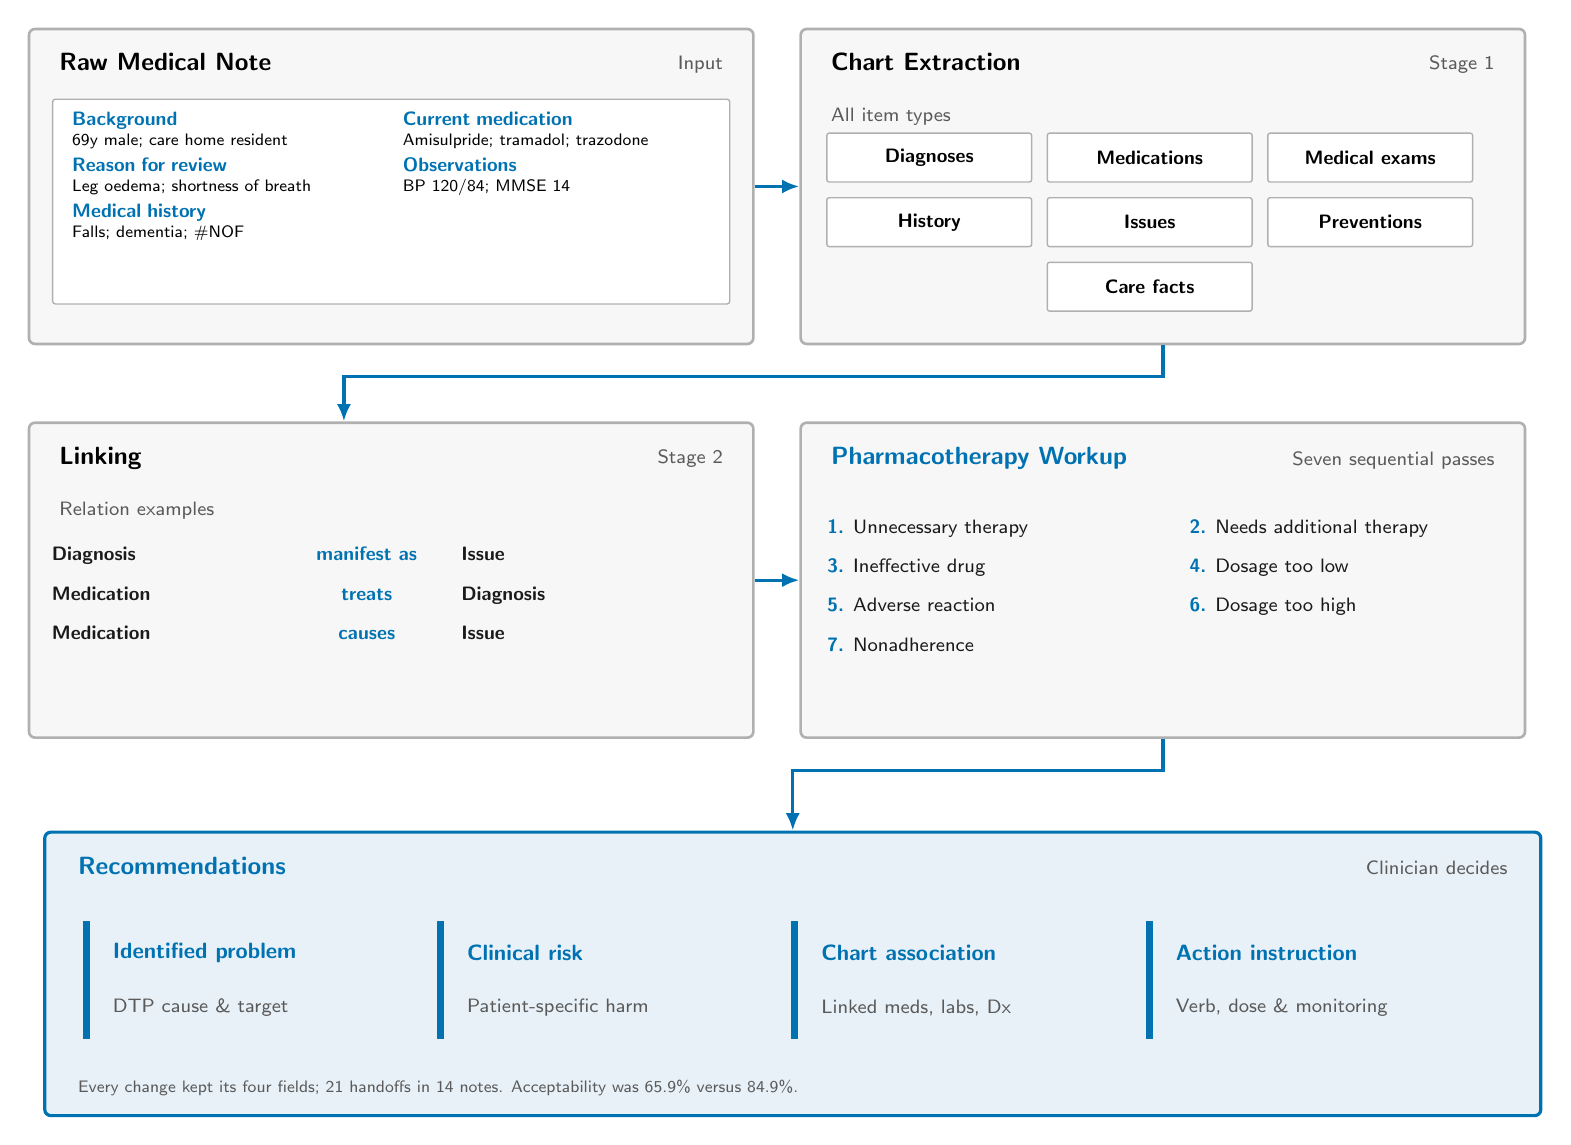
\begin{tikzpicture}[
  x=1mm, y=1mm,
  font=\fontsize{9}{11}\selectfont\color{cInk},
  >=Latex,
  stage/.style={
    draw=cLine, line width=0.95pt, rounded corners=2.2pt,
    fill=cCard, align=center, inner sep=0pt,
    minimum width=92mm, minimum height=40mm
  },
  stageout/.style={
    stage, draw=cBlue, line width=1.15pt, fill=cSoft,
    minimum width=190mm, minimum height=36mm
  },
  mainarr/.style={
    -{Latex[length=2.2mm,width=1.8mm]}, cBlue, line width=1.2pt
  },
  chip/.style={
    draw=cLine, line width=0.5pt, rounded corners=0.8pt, fill=white,
    font=\fontsize{6.8}{8}\selectfont\bfseries,
    inner xsep=0pt, inner ysep=1.2pt, align=center,
    minimum width=26mm, minimum height=6.2mm
  },
]

% Symmetric grid: 92 + 6 + 92 = 190 mm; row gap 10 mm
\node[stage] (c1) at (0,0) {};
\node[stage] (c2) at (98,0) {};
\node[stage] (c3) at (0,-50) {};
\node[stage] (c4) at (98,-50) {};
\node[stageout] (c5) at (51,-100) {};

% Shared title anchors (same inset on every card)
\newcommand{\cardtitle}[3]{%
  \node[font=\fontsize{9.5}{11}\selectfont\bfseries, anchor=north west]
    at ([xshift=2.8mm,yshift=-2.0mm]#1.north west) {#2};
  \node[font=\fontsize{7.5}{9}\selectfont\color{cMuted}, anchor=north east]
    at ([xshift=-2.8mm,yshift=-2.4mm]#1.north east) {#3};
}

% ---- Row 1 left: Raw Medical Note ----
\cardtitle{c1}{Raw Medical Note}{Input}
\node[draw=cLine, line width=0.5pt, rounded corners=1pt, fill=white,
      minimum width=86mm, minimum height=26mm, anchor=north]
  (note) at ([yshift=-9.0mm]c1.north) {};
% Two equal text columns with matching section margins
\node[anchor=north west, align=left, inner sep=0, text width=39mm,
      font=\fontsize{6.4}{7.6}\selectfont]
  at ([xshift=2.5mm,yshift=-1.6mm]note.north west) {%
    {\fontsize{6.8}{8}\selectfont\bfseries\color{cBlue}Background}\\[-0.05em]
    69y male; care home resident\\[0.28em]
    {\fontsize{6.8}{8}\selectfont\bfseries\color{cBlue}Reason for review}\\[-0.05em]
    Leg oedema; shortness of breath\\[0.28em]
    {\fontsize{6.8}{8}\selectfont\bfseries\color{cBlue}Medical history}\\[-0.05em]
    Falls; dementia; \#NOF%
  };
\node[anchor=north west, align=left, inner sep=0, text width=39mm,
      font=\fontsize{6.4}{7.6}\selectfont]
  at ([xshift=44.5mm,yshift=-1.6mm]note.north west) {%
    {\fontsize{6.8}{8}\selectfont\bfseries\color{cBlue}Current medication}\\[-0.05em]
    Amisulpride; tramadol; trazodone\\[0.28em]
    {\fontsize{6.8}{8}\selectfont\bfseries\color{cBlue}Observations}\\[-0.05em]
    BP 120/84; MMSE 14%
  };

% ---- Row 1 right: Chart Extraction (3x3 chip grid; last two empty) ----
\cardtitle{c2}{Chart Extraction}{Stage 1}
\node[font=\fontsize{6.6}{8}\selectfont\color{cMuted}, anchor=north west]
  at ([xshift=2.8mm,yshift=-9.0mm]c2.north west) {All item types};
\foreach \lab/\col/\row in {
  Diagnoses/0/0,
  Medications/1/0,
  Medical exams/2/0,
  History/0/1,
  Issues/1/1,
  Preventions/2/1,
  Care facts/1/2%
}{
  \node[chip] at ($(c2.north west)+(16.5mm+28mm*\col,-16.5mm-8.2mm*\row)$) {\lab};
}

% ---- Row 2 left: Linking (aligned three-column lines) ----
\cardtitle{c3}{Linking}{Stage 2}
\node[font=\fontsize{6.6}{8}\selectfont\color{cMuted}, anchor=north west]
  at ([xshift=2.8mm,yshift=-9.0mm]c3.north west) {Relation examples};
\node[anchor=north west, inner sep=0] at ([xshift=3.0mm,yshift=-15.5mm]c3.north west) {%
  \fontsize{7.4}{8.6}\selectfont
  \begin{tabular}{@{}>{\raggedright\arraybackslash}p{28mm}%
                 @{}>{\centering\arraybackslash}p{24mm}%
                 @{}>{\raggedright\arraybackslash}p{28mm}@{}}
  \textbf{Diagnosis} & \textcolor{cBlue}{\textbf{manifest as}} & \textbf{Issue} \\[2.0mm]
  \textbf{Medication} & \textcolor{cBlue}{\textbf{treats}} & \textbf{Diagnosis} \\[2.0mm]
  \textbf{Medication} & \textcolor{cBlue}{\textbf{causes}} & \textbf{Issue} \\
  \end{tabular}%
};

% ---- Row 2 right: Pharmacotherapy Workup (two equal columns) ----
\node[font=\fontsize{9.5}{11}\selectfont\bfseries\color{cBlue}, anchor=north west]
  at ([xshift=2.8mm,yshift=-2.0mm]c4.north west) {Pharmacotherapy Workup};
\node[font=\fontsize{6.8}{8}\selectfont\color{cMuted}, anchor=north east]
  at ([xshift=-2.8mm,yshift=-2.6mm]c4.north east) {Seven sequential passes};
\node[anchor=north west, inner sep=0] at ([xshift=3.5mm,yshift=-11.5mm]c4.north west) {%
  \begin{tabular}{@{}>{\fontsize{7.2}{8.5}\selectfont}p{42mm}%
                 @{\hspace{4mm}}%
                 >{\fontsize{7.2}{8.5}\selectfont}p{38mm}@{}}
  \textcolor{cBlue}{\textbf{1.}} Unnecessary therapy &
  \textcolor{cBlue}{\textbf{2.}} Needs additional therapy \\[1.1mm]
  \textcolor{cBlue}{\textbf{3.}} Ineffective drug &
  \textcolor{cBlue}{\textbf{4.}} Dosage too low \\[1.1mm]
  \textcolor{cBlue}{\textbf{5.}} Adverse reaction &
  \textcolor{cBlue}{\textbf{6.}} Dosage too high \\[1.1mm]
  \textcolor{cBlue}{\textbf{7.}} Nonadherence & \\
  \end{tabular}%
};

% ---- Row 3: Recommendations (four equal columns) ----
\node[font=\fontsize{9.5}{11}\selectfont\bfseries\color{cBlue}, anchor=north west]
  at ([xshift=3.2mm,yshift=-2.2mm]c5.north west) {Recommendations};
\node[font=\fontsize{7.5}{9}\selectfont\color{cMuted}, anchor=north east]
  at ([xshift=-3.2mm,yshift=-2.6mm]c5.north east) {Clinician decides};
% Four equal 45 mm columns inside 190 mm card (margins 5 mm each side)
\foreach \i/\title/\sub in {
  0/{Identified problem}/{DTP cause \& target},
  1/{Clinical risk}/{Patient-specific harm},
  2/{Chart association}/{Linked meds, labs, Dx},
  3/{Action instruction}/{Verb, dose \& monitoring}%
}{
  \pgfmathsetmacro{\fx}{5+45*\i}
  \fill[cBlue] ([xshift=\fx mm,yshift=-11.5mm]c5.north west) rectangle ++(0.9mm,-15mm);
  \node[font=\fontsize{8}{9.5}\selectfont\bfseries\color{cBlue}, anchor=west]
    at ([xshift=\fx mm+2.6mm,yshift=-15.5mm]c5.north west) {\title};
  \node[font=\fontsize{6.8}{8}\selectfont\color{cMuted}, anchor=west]
    at ([xshift=\fx mm+2.6mm,yshift=-22.5mm]c5.north west) {\sub};
}
\node[font=\fontsize{6.5}{7.6}\selectfont\color{cMuted}, anchor=south west, align=left]
  at ([xshift=3.2mm,yshift=1.5mm]c5.south west)
  {Every change kept its four fields; 21 handoffs in 14 notes. Acceptability was 65.9\% versus 84.9\%.};

% Flow: across, down-left, across, down to output
\draw[mainarr] (c1.east) -- (c2.west);
\draw[mainarr] (c2.south) -- ++(0,-4mm) -| ([xshift=-6mm]c3.north);
\draw[mainarr] (c3.east) -- (c4.west);
\draw[mainarr] (c4.south) -- ++(0,-4mm) -| (c5.north);

\end{tikzpicture}
\end{document}
